\documentclass[../main.tex]{subfiles}
\begin{document}
\chapter{AFM - SNOM}
Le immagini prese in esame in questa tesi sono state prodotte con un microscopio NeaSNOM. In questo capitolo viene descritta la sua struttura e le sue modalità di funzionamento...
\change{Imposta una introduzione quando finisci il capitolo}
\section{Storia della Microscopia}

I primi microscopi composti costruiti risalgono al 17\textdegree\ secolo, oltre 400 anni fa. È in quest'epoca che si riuscì a vedere per la prima volta i microrganismi che abitano la Terra ed ebbe inizio lo studio della Microbiologia. \textit{Robert Hooke} osservò le pareti cellulari e usò per la prima volta il termine ``cellula" \cite{fara_2009, micrographia}, mentre \textit{Antoine van Leeuwenhoek} sviluppò dei microscopi semplici (a singola lente) con ingrandimenti molto superiori a quelli degli strumenti contemporanei e fu il primo ad osservare microrganismi, come batteri e globuli rossi.\cite{lane_2015, dobell_1923, corliss_1975, jessup_2024}

\subsection{Microscopio ottico composto}

Il microscopio ottico composto ingrandisce l'immagine del campione usando delle lenti. il campione può essere illuminato facendolo attraversare dalla luce sul lato opposto all'obiettivo (microscopia a luce trasmessa) oppure riflettendocela sopra (microscopia a luce riflessa).

Il sistema più semplice è composto da due lenti, una lente obiettivo vicina al campione da esaminare, e una lente oculare vicina all'osservatore. Il campione è prima messo a fuoco dalla lente obiettivo dentro al microscopio in una immagine reale, poiché è creata dalla convergenza dei raggi di luce, poi questa immagine viene nuovamente ingrandita dalla lente oculare che crea una nuova immagine, stavolta virtuale visto che è creata da proiezioni di raggi divergenti. L'osservatore quindi vedrà un'immagine ingrandita, invertita e virtuale del campione esaminato.

\begin{figure}[h]
\centering
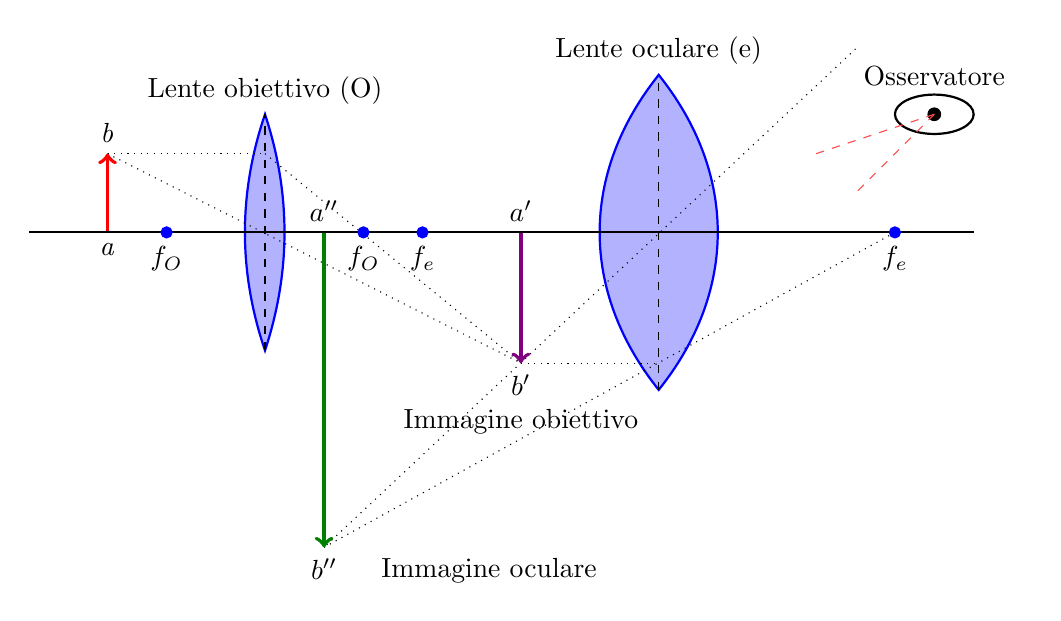
\begin{tikzpicture}
	% lente obiettivo
	\filldraw[thick,blue!30, draw=blue] (3,1.5) 
		.. controls (2.66,0.5) and (2.66,-0.5) .. (3,-1.5)
		.. controls (3.33,-0.5) and (3.33,0.5) .. cycle
		node[black,above] {Lente obiettivo (O)};
	\draw[dashed] (3,-1.5) -- (3,1.5);
	
	% lente oculare
	\filldraw[thick,blue!30, draw=blue] (8,2) 
	.. controls (9,0.75) and (9,-0.75) .. (8,-2)
	.. controls (7,-0.75) and (7,0.75) .. cycle
	node[black,above] {Lente oculare (e)};
	\draw[dashed] (8,-2) -- (8,2);
			
	\draw[dotted] (1,1) -- (3,1);
	\draw[dotted] (3,1) -- (6.25,-1.66);
	\draw[dotted] (1,1) -- (6.25,-1.66);
	
	\draw[dotted] (6.25,-1.66) -- (8,-1.66);
	\draw[dotted] (11,0) -- (3.75,-4);
	\draw[dotted] (10.5,2.33) -- (3.75,-4);
	
	% ogetto
	\draw[line width=0.5mm,Red,->] (1,0) node[below, black] {\textit{a}}
		-- (1,1) node[above, black] {\textit{b}};
	
	% immagine reale
	\draw[line width=0.5mm,Purple,->] (6.25,0) node[above, black] {$a'$}
		-- (6.25,-1.66) node[below, black, align=center] {$b'$ \\ \text{Immagine obiettivo}};

	% immagine virtuale
	\draw[line width=0.5mm,Green,->] (3.75,0) node[above, black] {$a''$}
		-- (3.75,-4) node[below, black] {$b''$} node[below right, black] {\ \ \quad Immagine oculare};

	% linea principale
	\draw[thick] (0,0) -- (12,0);
	
	% lungheazza focale lente oculare
	\filldraw[blue] (5,0) circle (2pt) node[below,black,inner sep=5pt]{$f_e$};
	\filldraw[blue] (11,0) circle (2pt) node[below,black,inner sep=5pt]{$f_e$};
	
	% lungheazza focale lente obiettivo
	\filldraw[blue] (1.75,0) circle (2pt) node[below,black,inner sep=5pt]{$f_O$};
	\filldraw[blue] (4.25,0) circle (2pt) node[below,black,inner sep=5pt]{$f_O$};
	
	% occhio
	\draw[thick] (11.5,1.5) ellipse (0.5 and 0.25)
		node[above, inner sep=10pt] {Osservatore};
	
	% pupilla
	\filldraw[black] (11.5,1.5) circle (0.08);
	
	% raggi visivi
	\draw[red!70, dashed] (11.5,1.5) -- (10,1);
	\draw[red!70, dashed] (11.5,1.5) -- (10.5,0.5);
\end{tikzpicture}
\caption{Principio di funzionamento di un microscopio ottico composto}
\label{fig:com_diag}
\end{figure}

Il microscopio ottico composto ha continuato ad essere sviluppato fino ad oggi e ne sono state create molte varianti per scopi più specializzati, come il microscopio a contrasto di fase (\acrshort{pcm})\cite{zernike_1955} o il microscopio confocale (\acrshort{clsm})\cite{pawley_2006}. In generale, oggi la microscopia ottica ha raggiunto altissimi livelli di prestazioni, sia ottiche che meccaniche, ma la cui risoluzione spaziale è rimasta bloccata dal limite di diffrazione della luce.

\subsection{Apertura numerica}

Il primo a definire questo limite fu \textit{Ernst Abbe} nel 1881, anno in cui pubblicò il suo lavoro sulla misura dell'apertura dei microscopi.\cite{abbe_1881} Questo limite, chiamato apertura numerica (\acrshort{na}), descrive l'intervallo degli angoli della luce che il microscopio può accettare ed è comunemente usato in microscopia come parametro delle ottiche per valutarne la risoluzione. Questo numero è definito come il prodotto tra l'indice di rifrazione \textit{n} e il seno dell'apertura angolare della lente.

\begin{equation}
	NA=n\sin\theta
\end{equation}

Da questa formula, \textit{Abbe} continuò il suo lavoro arrivando a definire anche la minima distanza tra elementi diversi affinchè si possano apprezzare attraverso un microscopio.\cite{abbe_1882}

\begin{equation}
d=\frac{\lambda}{2NA}=\frac{\lambda}{2n\sin\theta}
\end{equation}

Usando l'aria come mezzo di trasmissione si ha un indice di rifrazione di 1, mentre si può arrivare fino a circa 1.5 immergendo il campione e l'obiettivo in olio. Per quanto riguarda l'apertura angolare massima,  teoricamente può arrivare fino a 180\degree, il che si traduce in un valore di $\theta=90$\degree, ma ad ora le lenti con la più alta apertura angolare mai realizzate si fermano approssimativamente a 144\degree, che corrisponde a un valore di $\sin\left(\theta=72\degree\right) \approx 0.95$.\cite{leica_aperture}

Per migliorare la risoluzione oltre il limite dei 200nm, ottenibili usando lunghezze d'onda dello spettro visibile, bisogna scegliere raggi a lunghezza d'onda minore, come i raggi X o UV. Queste tecniche portano una risoluzione maggiore ma anche delle controindicazioni, come una scarsa risposta da parte del campione oppure tossicità.

\subsection{Microscopio elettronico}

\section{AFM}

\section{SNOM}

\section{Batteri}

\end{document}
